\section{ Description of classes. }
%
\subsection{ Classes for input and output data}
\begin{itemize}
%
\item{ Class {\bf DefineInOutFiles}} \\
\begin{print}
In this class we define auxiliary files, such as {\it trace }-file (file,where we list all methods and classes, which were used during running of program; this file should help developer to trace a mistake), {\it debug}-file (file, where intermediate results are stored), {\it info} - file (in this file we print specific information about methods and types of data, which were used in code)
\end{print}
%
\item{ Class {\bf FileType}} \\
\begin{print}
Base class for reading input data. Its function is virtual due to handle the different types of input files and to hide their features from developer of code.
\end{print}
%
\item{ Class {\bf DatFile}} \\
\begin{print}
This class is derived from class FileType. It reads necessary data from {\it dat} - file, which is produced by CAPAPRE.
\end{print}
%
\item{ Class {\bf Material}} \\
\begin{print}
This class contains methods for reading information about material from special file, which contains data about it. In future we plan to implement here also methods for the interpolation / approximation of nonlinear material behaviour, transformations of material tensors as well as the handling of inhomogeneous material data.
\end{print}
%
\item{ Class {\bf TimeFunc}} \\
\begin{print}
This class stores information about given time function. Later it should provide methods for handling time functions, interpolation (1D, 2D, 3D) of initial and load (nodal-, surface-, volume-type) data.\\
{\em Input: } FileType \\
\end{print}
%
\item{ Class {\bf OutResultUnverg}} \\
\begin{print}
Organization of classes for output result is the same as for input data. This class is derived from a base class OutResult.
It provides methods for output result in {\it unverg }- format. \\ 
{\it Input: } Driver \\
\end{print}
\end{itemize}
%
\subsection{ Classes for handling grids on calculation domain} 
%
\begin{itemize}
%
\item{ Class {\bf Grid}} \\
\begin{print}
This class contains methods for working with grid. For each level of refinement we create structure {\it GridHierarchy}, which stores all information about grid, such as maximum number of elements and nodes, type of each element, its connection, coordinates of nodes.    
\end{print}
%
\item{ Class {\bf Domain}} \\
\begin{print}
This class contains information about calculation domain. In this class we define subdomains, which correspond to different material regions as well as equations and , correspondingly, can have different discretization. For each subdomain a object of class Grid is allocated. It's possible situation, when on the same physical domain we have different discretization (e.g. coupled field problem, different discretization for mechanic and magnetic field), therefore different objects of class Grid for the same subdomain should be created.
\end{print}
\end{itemize}
\subsection{ Classes for defining finite element spaces }
\begin{figure}[H]
\begin{center}
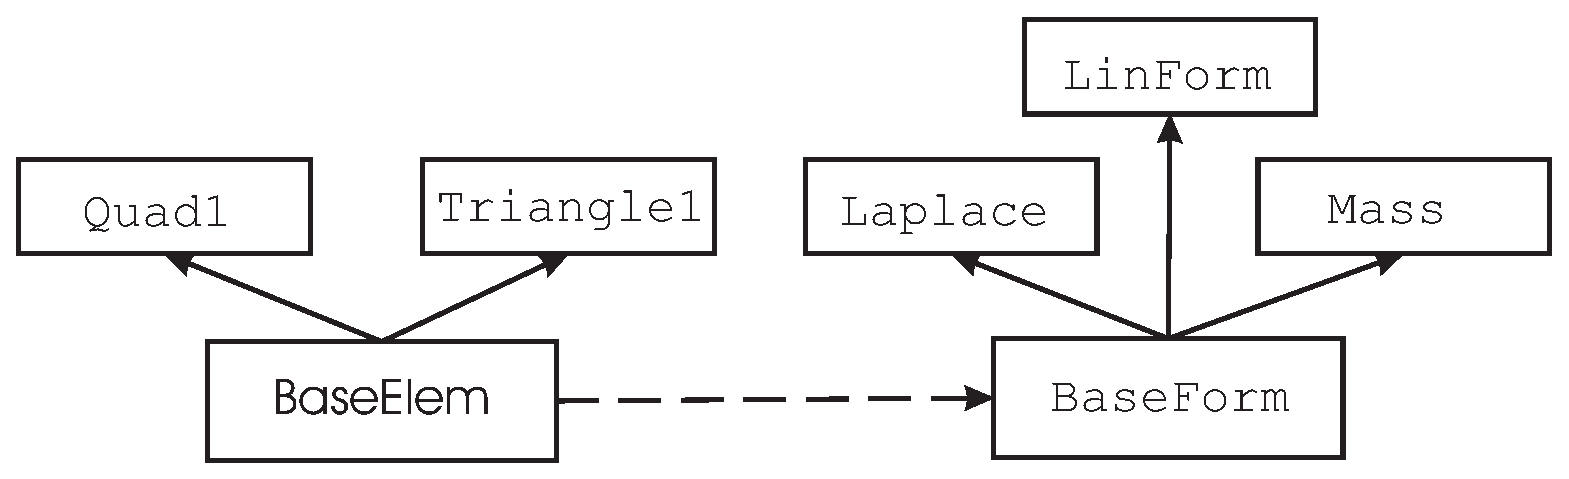
\includegraphics [width=8cm, angle=0] {./pic/baseform1}
\end{center}
\caption{ Interaction between classes BaseElem and BaseForm } 
\end{figure}
\begin{itemize} 
\item{ Class {\bf BaseElem}} \\
\begin{print}
 This is a base class for description of finite element. In this class we define following attributes of finite element: dimension, number of nodes, number of edges, number of faces, number of integration points, integration points themself and appropriate integration weights. It stores virtual function for initialization information about finite element, set integration points, calculation of shape function and its derivatives at these points. 
These functions are substituted by specific functions in derived classes.
\end{print}
\item{ Classes {\bf Quad1, Triangle1, Quad2, Triangle2 }} \\
\begin{print}
 These classes are derived from BaseElem and contained specific information about , accordingly, bilinear quadrilateral, linear triangle, quadratic quadrilateral, quadratic triangle element and so on. 
\end{print}
\end{itemize}
\subsection{ Classes for calculation the element matrices}
\begin{itemize}
%
\item{ Class {\bf BaseForm}} \\
\begin{print}
 This class is a base class for computing the element matrices in accordance with form  
\begin{eqnarray*}
\int {\bf B}^{\it T}{\bf D}{\bf B} \; dx
\end{eqnarray*}
, where {\bf B} is differential operator and {\bf D} the material tensor.
 It provides methods for computation of element matrix on given element, type of which we define in constructor through the pointer to BaseElem. Main members of this class are functions for computing element matrix for different combination of shape function and its derivatives. For this purpose auxiliary functions, such as calculation of transformation given element in standard one, calculation of determinate of this transformation, are implemented. The virtual function CalcElemMatrix in this class is overloaded in each derived class. \\    
{\it Input: } BaseElem \\
{\it Output: } Assemble
\end{print} 
%
\item{ Class {\bf LaplaceInt}}\\
\begin{print}
 This class is derived from class BaseForm for computation element stiffness matrix of laplace operator. This can be done by using main member of this class {\sf CalcElemMatrix}.
\end{print}
%
\item{ Class {\bf MassInt}}\\
\begin{print}
 This class is analogous to class LaplaceInt, only method {\sf CalcElemMatrix} computes element mass matrix.
\end{print}
\end{itemize} 
%
\subsection{ Classes for assembling and solving system matrix }
\begin{itemize}
%
\item{ Class {\bf SystemMatrix}} \\
\begin{print}
 This class stores system matrix and right hand side arising from finite element discretization. It is base class for classes LinSystem and Assemble. It is done that way in order to store these data once in program and there is
 explicit access to them from methods of classes LinSystem and Assemble. This class is implemented as template. Owing to that fact, we can define type of system matrix( sparse, symmetric or band matrix), when we determine object of the class. 
\end{print}
%
\item{ Class {\bf Assemble}} \\
\begin{print}
This class provides methods for assembling global system matrix according to the weak form of the differential equations. \\
{\it Input: } Grid 
\end{print}
%
\item{ Class {\bf LinSystem}} \\
\begin{print}
 This class provides methods for solving linear algebraic system. At present Conjugate Gradiate method and BiCGSTAB method are implemented. This class is derived from class SystemMatrix, so it works with matrix and right hand side, which are stored in it. 
\end{print}
%
\item{ Class {\bf WorkWithSystemMatrix}} \\
\begin{print}
 This class is derived from class LinSystem and Assemble. It is created only with aim to have for classes LinSystem and Assemble the same base class SystemMatrix.
\end{print}
\end{itemize}
%
\subsection{ Specific classes for regarding problem }
\begin{itemize}
\item { Class {\bf Driver}} \\
\begin{print}
The main element in the code organization is class Driver. It is a base class. In this class we conduct time-stepping. Due to this fact we conduct error estimation and refinement of grid in this class. In addition, the special algorithms concerned the coupling procedure of the different single field problems will be handled thereby. Constitutive action of this class are initialization derived classes from PDE in accordance with regarding problem, for example AcousticPDE, and define grid, on which this differential equation should be solved. Additionally, in this class we 
cause object of class {\sf OutResultUnverg}  for output of resultes.\\
{\em Input: } FileType, Material \\
{\em Output: } OutResultUnverg 
\end{print}
%
\item{ Class {\bf PDE}} \\
\begin{print}
Class PDE is base class, from which classes for different type of PDE are derived.
This class contains general things for different types of equations, for example, data about integration parameters, method to calculate parameters for Newmark method. \\
{\em Input: } FileType, Material \\
\end{print}
%
\item{ Class {\bf AcousticPDE} } \\
\begin{print}
This class is derived from class PDE. It is used for solving acoustic equation on one time step. 
In this class we work with complex WorkWithSystemMatrix. When we create object of this class , we determine what kind of matrix should be system matrix, for example, sparse matrix, band matrix, symmetric matrix. We set rules for assembling global system matrix according to weak form of partial differential equation, define right hand side and set boundary conditions. Then we cause one of methods of LinSystem for solving linear system. On the last step we calculate first and second derivatives of the solution. \\ 
{\em Input: } Grid, TimeFunc \\
{\em Output: } WorkWithSystemMatrix 
\end{print}
%
\end{itemize}
%
\subsection{ Useful tools }
\begin{itemize}
\item{ Class {\bf Vector}} \\
\begin{print}
 This class is defined for working with arrays of different data types. It stores pointer to allocated array and its size. A lot of functions, such as multiplication, algebraic operation, resize, cut element, put element and so on, are implemented. Merit of this class is that we needn't deallocate arrays ourself, this job would be done automatically by deconstructor. This class is implemented as simple template class with parameter - data type.  
\end{print}
%
\item{ Class {\bf AbsMatrix}} \\
\begin{print}
 It is a base class for different types of matrices. Principles of organization of storage matrix is similar for all types of matrices. The data of a matrix are allocated as a one contigues memory block and there are pointers to the first element of each row. At present the following types of matrix are implemented: 
 \begin{itemize}
 \item[-] full matrix (class {\bf Matrix}), 
 \item[-] symmetric matrix (class {\bf SymMatrix}), 
 \item[-] sparse matrix (class {\bf SparseMatrix}), 
 \item[-] symmetric sparse matrix (class {\bf SymSparseMatrix}), 
 \item[-] band matrix ( class {\bf BandMatrix}), 
 \item[-] symmetric band matrix ( class {\bf SymBandMatrix}), 
 \end{itemize}
All these classes are derived from AbsMatrix. Each of these classes contains overloading algebraic operations, operation for output results in file or screen, cut or put elements in matrix, methods for resize and allocation matrix. Additionally, such function as precondition of matrix, is put in these classes. Due this fact class {\sf LinSystem} is independent from type of matrix, so we can use it as parameter in template of its.  At present Jacobi, 
SSOR percondition type are implemented.
 For sparse matrix we use CRS( Compressed Row Storage) storage scheme.
Lately we discuss one detail of implementation of hierarchy of this classes.
\end{print}
%
\item{ Class {\bf Clock}}\\
\begin{print}
 This class provides tools for timing program.
\end{print}
\item{ Class {\bf Error}}\\
\begin{print}
 Members of this class are used for informing user about mistake during runtime of program. 
\end{print}
\end{itemize}
